\documentclass[APA,STIX1COL]{WileyNJD-v2}
\usepackage[utf8]{vietnam}
\graphicspath{ {Figs/} } 
\articletype{FOBE}

\received{30 Sep 2022}
\revised{5 Oct 2022}
\accepted{5 Oct 2022}

\raggedbottom

\begin{document}

\title{Assignment 3\protect\thanks{Supervisor: Tran Manh Hung.}}

\author[1]{Nguyen Hoang Tan}

\author[2]{Le Gia Khang}

\author[3]{Lê Thị Kim Yến}



\authormark{FOBE}


\address[1]{\orgname{Hoang Tan}, \country{Question 1,4}}

\address[2]{\orgname{Gia Khang}, \country{Question 2}}

\address[2]{\orgname{Kim Yến}, \country{Question 3}}


\corres{*\email{21521413@gm.uit.edu.vn} \\ *\email{21522189@gm.uit.edu.vn} \\ *\email{21521695@gm.uit.edu.vn} \\ \\ IT005.N12.KHCL - University of Information Technology}


\abstract[Summary]{Định nghĩa và so sánh TCP, UDP \\ So sánh HTTP bền vững và HTTP không bền vững \\ Sự giống và khác nhau của Pop 3 và Imap \\ Tìm hiểu DNS là gì và tại sao phải đung DNS, phân tích một vài DNS hiện có}

\keywords{TCP, UDP, HTTP, Pop 3, Imap, DNS}


\maketitle



\section{So sánh TCP và UDP}\label{sec1}
\subsection*{*Định nghĩa}
\begin{itemize}
  \item TCP (Transmision Control Protocol) là một trong những giao thức chính của bộ giao thức Internet. Nó nằm giữa tầng Application và Network, được sử dụng để cung cấp các dịch vụ vận chuyển (delivery) đang tin cậy. Đây là một giao thức định hướng kết nối (Connection-Oriented)
để rao đổi thông tin giữa các thiết bị trng hệ thống mạng.
  \item UDP (User Datagram Protocol) là một giao thức thuộc tầng Transport. UDP là một giao thức
truyền thông được sử dụng trên Internet để truyền tải những dẫn truyền nhạy cảm về thời gian như phát lại
video hoặc tra cứu DNS
\end{itemize}

\begin{figure}[h]
  \centering
  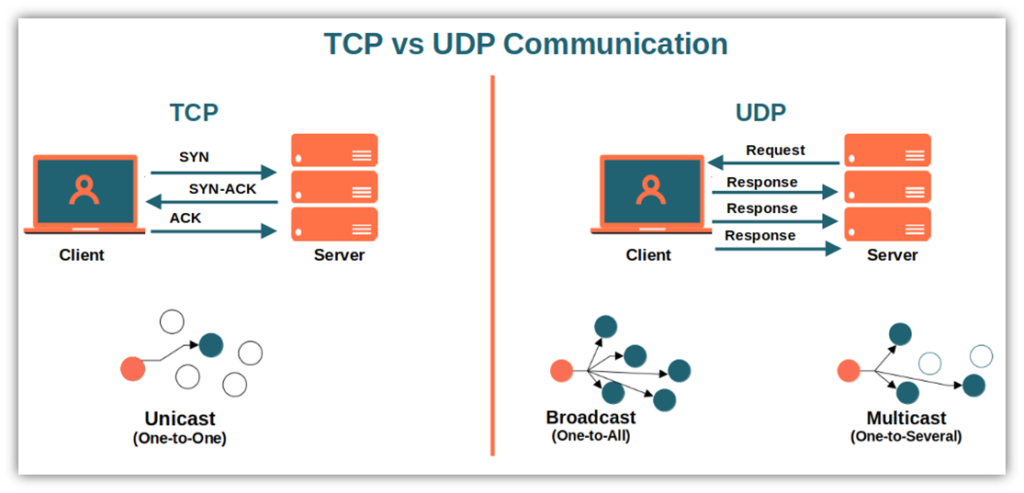
\includegraphics[scale=0.3]{tcp_udp}
  \caption{TCP and UDP Communication}
  \label{fig:tcpvsudp}
\end{figure}



\begin{center}
  \begin{table}[t]%
  \centering
  \caption{*So sánh TCP và UDP.\label{tab2}}%
  \begin{tabular*}{500pt}{@{\extracolsep\fill}lcccc@{\extracolsep\fill}}
  \toprule
  \textbf{Basis} & \textbf{TCP}  & \textbf{UDP} \\
  \midrule
  Loại dịch vụ & Connection-Oriented  & Datagram-Oriented     \\
  Độ tin cậy & Đáng tin cậy  & Không đáng tin cậy  \\
  Cơ chế kiểm tra lỗi & Cung cấp các cơ chế kiểm tra lỗi mở rộng  & Cơ chế kiểm tra lỗi cơ bản  \\
  Tốc độ & TCP tương đôí chậm hơn UDP & UDP nhanh hơn, đơn giản hơn và hiệu quả hơn UDP \\
  Broadcasting & Không hỗ trợ & Hỗ trợ \\
  Giao thức & HTTP, HTTPs, FTP, SMTP và Telnet & DNS, TFTP, RTSP, SNP \\
  Luồng & byte & message \\


  \bottomrule
  \end{tabular*}
  \begin{tablenotes}
  \item Ứng dụng: Nên lựa chọn loại giao thức nào:
  \item[$\dagger$] TCP: được dùng khi các gói dữ liệu được gửi theo thứ tự.
  \item[$\ddagger$] UDP: được dùng đói với live video, audio game online ( ưu tiên tốc độ ).
  \end{tablenotes}
  \end{table}
  \end{center}


  \begin{figure}[h]
    \centering
    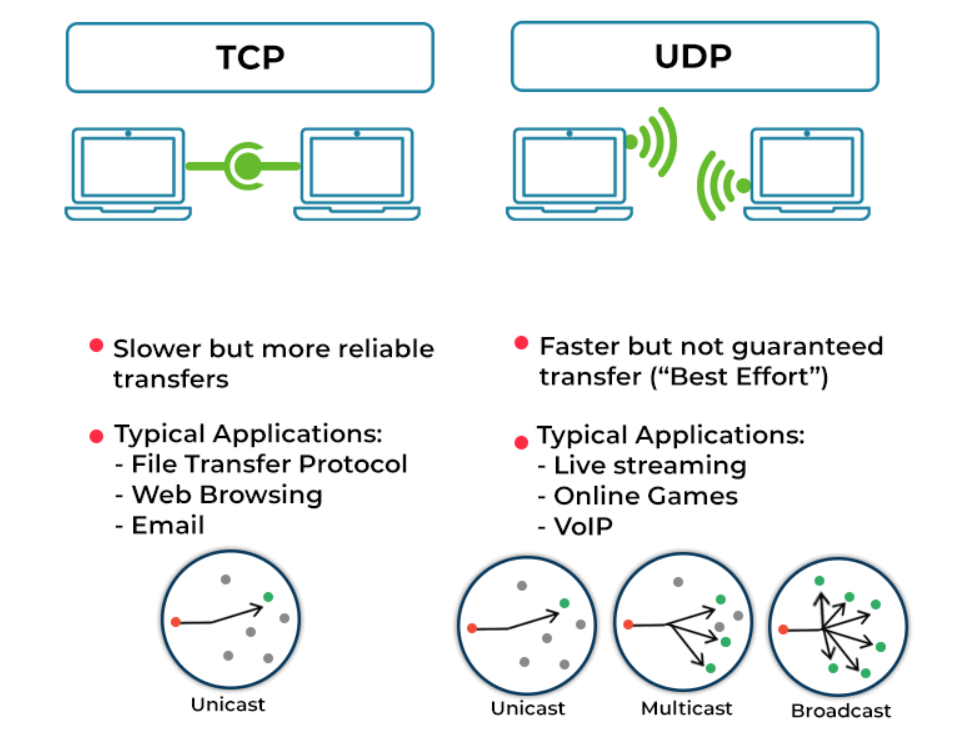
\includegraphics[width=15cm]{tcp_udp_1}
    \caption{TCP vs UDP Communication}
    \label{fig:tcpvsudp1}
  \end{figure}

\section{HTTP}\label{sec2}
\subsection*{*Định nghĩa HTTP}
Hypertext Transfer Protocol (HTTP) là giao thức thuộc lớp ứng dụng web. Sử dụng kết nối TCP cổng 80. HTTP được định nghĩa trong RFC 1945 (HTTP 1.0) và RFC 2616 (HTTP 1.1).

\begin{figure}[h]
  \centering
  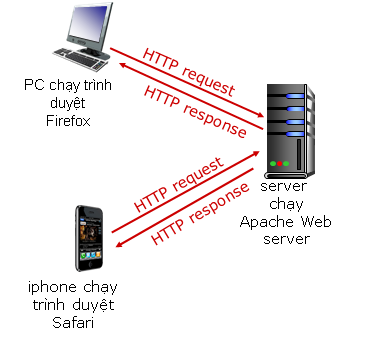
\includegraphics[scale=0.7]{http}
  \caption{Mô hình client-server}
  \label{fig:http}
\end{figure}

\subsection*{*Kết nối HTTP}
Có hai loại kết nối HTTP là kết nói không bền vững và kết nối bền vững. \\

HTTP không bền vững:
\begin{itemize}
  \item Chỉ tối đa một đối tượng được gửi qua 1 kết nối TCP, kết nối sau đó sẽ bị đóng;
  \item HTTP 1.0;
  \item Yêu cầu 2 RTT cho một gói tin;
  \item Trình duyệt mở song song nhiều kết nối TCP đến các đối tượng được quan tâm.
\end{itemize}

HTTP bền vững:
\begin{itemize}
  \item Nhiều đối tượng được gửi qua 1 kết nối TCP. Server giữ trạng thái mở sau khi gởi response;
  \item HTTP 1.1;
  \item Được chia ra 2 loại không có pipelining và có pipelining;
\end{itemize}

\begin{figure}[h]
  \centering
  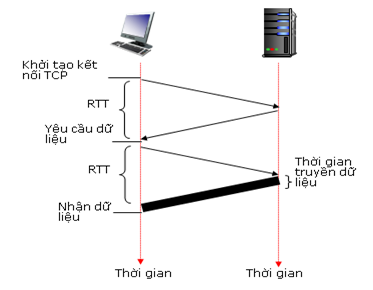
\includegraphics[scale=0.7]{http_1}
  \caption{Quy trình hoạt động kết nối HTTP không bền vững}
  \label{fig:http_1}
\end{figure}





\section{Pop3 và Imap}\label{sec3}
\subsection*{*Định nghĩa Pop3}
POP3 (Post Office Protocol version 3) là giao thức được sử dụng để kết nối tới server email và tải email xuống máy tính cá nhân. POP3 là một giao thức cũ hơn, ban đầu được thiết kế để chỉ sử dụng trên một máy tính. Không giống như các giao thức hiện đại sử dụng đồng bộ hóa hai chiều, POP3 chỉ hỗ trợ đồng bộ hóa email một chiều, chỉ cho phép người dùng tải email từ server đến client.
\begin{figure}[h]
  \centering
  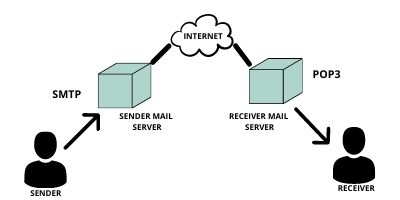
\includegraphics[scale=0.7]{POP3}
  \caption{Cách hoạt động của POP3}
  \label{fig:pop3}
\end{figure}



POP có hai bản sửa đổi bổ sung một số cải tiến: POP2 và POP3 được giới thiệu trong những năm sau đó. Hiện tại, POP3 vẫn là phiên bản hoàn chỉnh mới nhất của giao thức.
\subsubsection*{Ưu điểm}
\begin{itemize}
  \item POP3 được ưa chuộng vì tính đơn giản;
  \item Cho phép truy xuất email một cách hiệu quả và ít xảy ra lỗi;
  \item POP3 rất lý tưởng cho người dùng cần truy cập email của họ ngoại tuyến và sử dụng thiết bị được chỉ định để truy xuất. POP3 cũng rất hữu ích để gửi và lưu trữ các thư email hàng loạt;
  \item POP3 yêu cầu ít bộ nhớ hơn vì tất cả các email được lưu trữ trên PC cục bộ.
\end{itemize}

\subsubsection*{Nhược điểm}
\begin{itemize}
  \item Thư mục email có thể bị hỏng hoặc bị mất hoàn toàn, quá trình khôi phục mất nhiều thời gian;
  \item Email đính kèm có thể chứa virus và đe dọa đến toàn bộ máy tính nếu việc quét virus không được thực hiện đúng cách;
  \item Chiếm nhiều không gian trống vì tất cả thử được lưu trên ổ cứng;
  \item Không hỗ trợ đồng bộ hóa email trên server, vì email sau khi được tải xuống client sẽ bị xóa khỏi máy chủ.
\end{itemize}


\subsection*{*Định nghĩa IMAP}
IMAP (Internet Message Access Protocol) cho phép truy cập email từ nhiều thiết bị khác nhau. IMAP thực hiện điều này bằng cách giữ dữ liệu email được lưu trữ trên server, thay vì máy của người dùng. Khi một thiết bị truy cập vào tài khoản email, server sẽ lấy thông tin cập nhật cho thiết bị.
\begin{figure}[h]
  \centering
  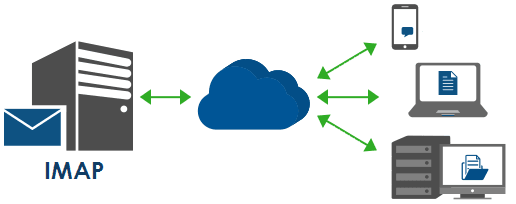
\includegraphics[scale=0.5]{imap}
  \caption{Cách hoạt động của imap}
  \label{fig:imap}
\end{figure}

IMAP được ra mắt vào năm 1986 bởi Mark Crispin như một giao thức truy cập từ xa, trái ngược với POP được sử dụng rộng rãi, IMAP chỉ đơn giản là lấy nội dung của thư. IMAP đã trải qua một số phiên bản trước version 4rev1 (MAP4) hiện nay, gồm IMAP ban đầu, IMAP2, IMAP3, IMAP2bis, IMAP4.

\subsubsection*{Ưu điểm}
\begin{itemize}
  \item Tải xuống nhanh hơn;
  \item Cho phép truy cập email từ mọi nơi, thông qua nhiều thiết bị khác nhau;
  \item Mail được tự động sao lưu;
  \item Tùy chọn lưu trữ cục bộ;
  \item Tiết kiệm dung lượng lưu trữ cục bộ;
  \item Xem nhanh hơn khi chỉ có các tiêu đề mail được tải về đến khi nội dung được yêu cầu rõ ràng.
\end{itemize}

\subsubsection*{Nhược điểm}
\begin{itemize}
  \item Cần kết nối Internet để hoạt động;
  \item Mở các file đính kèm chậm hơn.;
  \item Một số máy chủ email sẽ tính phí để cung cấp IMAP dưới dạng tùy chọn;
  \item Nếu sử dụng email để xử lý công việc nhiều thì qua thời gian sẽ bị đầy và không nhận hay gửi email được nữa.
\end{itemize}

\subsection*{*So sánh POP3 và IMAP}
IMAP và POP3 đều là hai phương pháp để truy nhập email.
\begin{figure}[h]
  \centering
  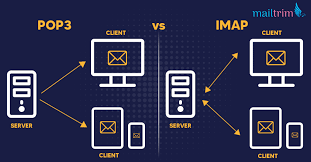
\includegraphics[scale=1]{imapvspop3.png}
  \caption{Pop3 vs IMAP}
  \label{fig:imapvpop3}
\end{figure}

\begin{center}
  \begin{table}[h]%
  \centering
  \caption{*Sự khác nhau giữa Pop3 và IMAP.\label{tab2}}%
  \begin{tabular*}{500pt}{@{\extracolsep\fill}lcccc@{\extracolsep\fill}}
  \toprule
  \textbf{POP3}  & \textbf{IMAP} \\
  \midrule
  Đây là một giao thức đơn giản . & IMAP nâng cao hơn nhiều. \\
  Kết nối trên port 110 . & Kết nối trên port 143. \\
  Có bảo mật SSL (POP3DS) kết nối trên port 995 & Có bảo mật SSL (IMAPDS) kết nối trên port 993. \\
  Mỗi lần chỉ có thể truy cập từ một thiết bị duy nhất. & Tin nhắn có thể được truy cập trên nhiều thiết bị. \\
  Phải tải thư xuống hệ thống cục bộ để đọc. & Nội dung thư có thể được đọc một phần trước khi tải xuống. \\
  Người dùng không thể tạo, xóa hoặc đổi tên email. & Người dùng có thể tạo, xóa hoặc đổi tên email. \\
  Có thể thay đổi thư bằng phần mềm email cục bộ. & Các thay đổi đã thực hiện trên web vẫn đồng bộ với máy chủ. \\
  Tất cả tin nhắn được tải xuống cùng một lúc. & Tiêu đề tin nhắn có thể được xem trước khi tải xuống. \\
  Có thể hoạt động không cần kết nối Internet. & Cần kết nối Internet để hoạt động \\
  Email chủ yếu lưu trên máy của người dùng. & Email chủ yếu lưu trên máy chủ. \\
  Nhanh hơn IMAP. & Chậm hơn POP3. \\
  \bottomrule
  \end{tabular*}

  \end{table}
  \end{center}


\section{DNS}
\subsection*{*DNS là gì ?}
DNS (Domain Name System) - hệ thống phân giải tên miền, là một trong những thành phần dễ bị nhầm lẫn nhất trong mô hình web. DNS giúp kết nối các tên miền với các web server. Nói các khác, nó chuyển những tên miền dễ hiểu với con người như google.com rồi chuyển nó thành địa chỉ IP dễ hiểu với máy tính.

\begin{figure}[h]
  \centering
  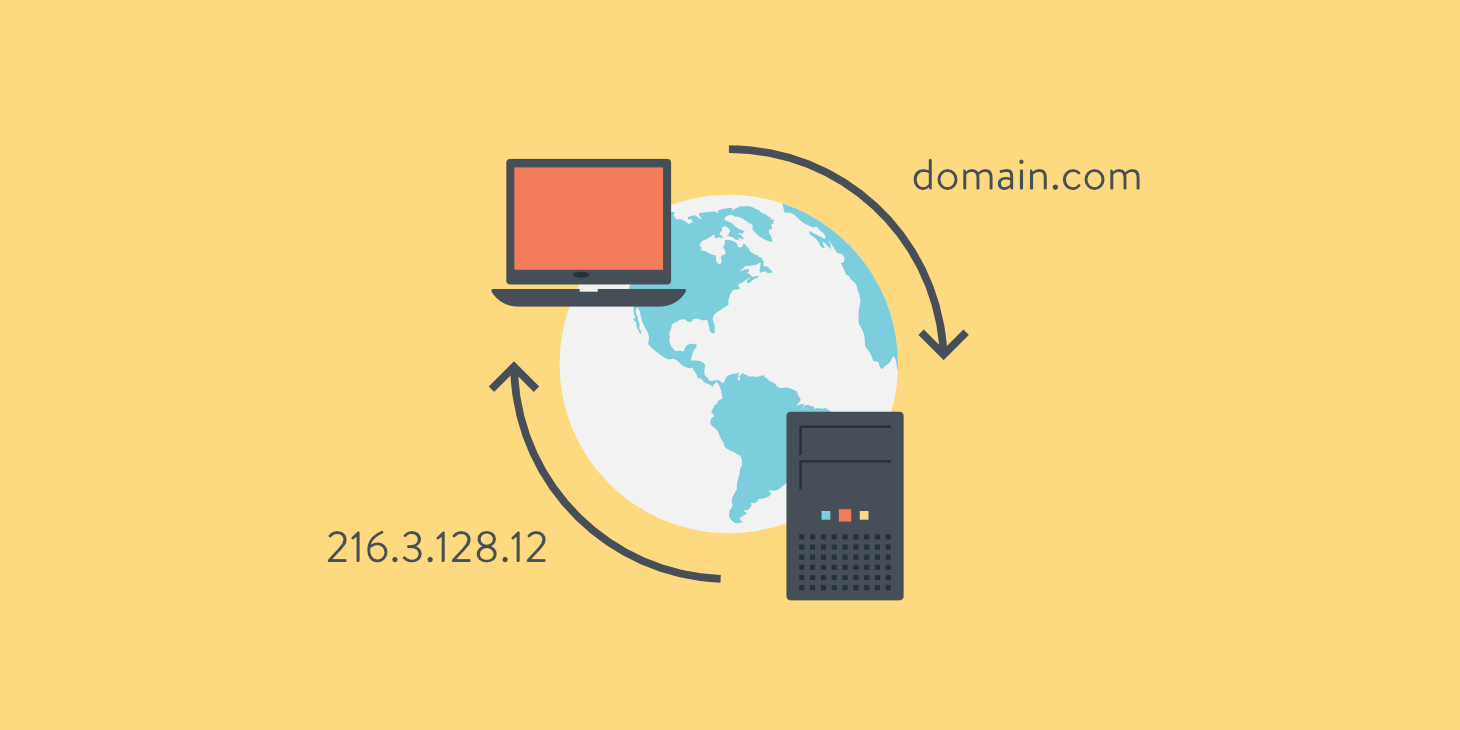
\includegraphics[scale=0.2]{dns}
  \caption{Domain Name System}
  \label{fig:imap}
\end{figure}

\subsection*{*Vì sao phải dùng DNS}
Trước đây, mỗi lần truy cập vào website người ta cần phải ghi nhớ chính xác các địa chỉ phức tạp và khó hiểu. Tuy nhiên, hệ thống DNS ra đời đã xoá tan đi gánh nặng đó. \\

Với tính năng ghi nhớ những tên miền đã được “dịch” và ưu tiên sử dụng cho những lần truy cập sau, DNS giúp người dùng tiết kiệm rất nhiều thời gian khi truy cập vào những website đã từng sử dụng.\\

Có thể nói không có DNS, Internet sẽ mau chóng lụi tàn để bạn có thể hình dung về mức độ quan trọng của DNS.
\subsection*{*Các loại DNS hiện có}
\begin{itemize}
  \item DNS Records: CNAME, A, MX, AAAA, TXT, SRV, NS;
  \item DNS Servers: Root Name Server, Local Name Server;
  \item DNS Queries: recursive, iterative, and non-recursive;
\end{itemize}


\section{Reference}
\begin{enumerate}
  \item \href{https://support.microsoft.com/vi-vn/office/imap-v%C3%A0-pop-l%C3%A0-g%C3%AC-ca2c5799-49f9-4079-aefe-ddca85d5b1c9
  }{support.microsoft.com/vi-vn/office/imap}
  \item \href{https://vietnix.vn/pop3-va-imap-la-gi/#:~:text=POP3%20ch%E1%BB%89%20l%C6%B0u%20tr%E1%BB%AF%20c%C3%A1c,%C4%91%E1%BA%A1i%20v%C3%A0%20linh%20ho%E1%BA%A1t%20h%C6%A1n.}{vietnix.vn}
  \item \href{https://quantrimang.com/cong-nghe/phan-biet-pop-va-imap-89580
  }{quantrimang.com}
\end{enumerate}

\end{document}
